% ============================================================
%  SUPPLEMENTARY MATERIAL
%  Physics of Fluids submission — Wolff et al.
%
%  Compilar por separado del manuscrito principal.
%  Numeracion independiente: FIG. S1, TABLE S1, Eq. (S1).
% ============================================================
\documentclass[%
  aip,
  pof,
  reprint,
  floatfix
]{revtex4-2}

\usepackage{graphicx}
\usepackage{amsmath}
\usepackage{amssymb}
\usepackage{bm}
\usepackage{siunitx}
\usepackage{booktabs}
\usepackage{multirow}
\usepackage{xcolor}
\usepackage{makecell}
\usepackage{hyperref}

\newcommand{\todo}[1]{\textcolor{red}{\textbf{[TODO: #1]}}}

% ── Atajo para p-values en notacion cientifica ──────────────
\newcommand{\pv}[2]{$#1{\times}10^{#2}$}

% ── Numeracion suplementaria ────────────────────────────────
\renewcommand{\thesection}{S\arabic{section}}
\renewcommand{\thefigure}{S\arabic{figure}}
\renewcommand{\thetable}{S\arabic{table}}
\renewcommand{\theequation}{S\arabic{equation}}

\begin{document}

\title{Supplementary material for\\
``A numerical reduced model for fiber orientation prediction in unsteady viscoplastic flows, from experimental PIV and PTV on Carbopol''}

\author{Lukas Wolff}
\author{Sebasti\'an Sep\'ulveda}
\author{Crist\'obal Maggi}
\author{Juan Pablo Toro}
\author{Jorge G\'omez}
\author{\'Alvaro Paul}
\author{Patricio A.\ Moreno-Casas}
\email{patriciomoreno@miuandes.cl}
\affiliation{%
  Facultad de Ingenier\'ia y Ciencias Aplicadas,
  Universidad de los Andes, Santiago, Chile
}

\maketitle

\noindent
This document collects the procedures, parameters and secondary analyses referred to in the main text. It is organized in the order in which the main text invokes it: the derivation of the saturation law (Sec.~\ref{sup:derivation}), the complete geometry of the casting device (Sec.~\ref{sup:geometry}), the record of the gel preparation (Sec.~\ref{sup:carbopol}), the processing parameters of the two optical techniques and the computational saving their block structures achieve (Secs.~\ref{sup:piv} to~\ref{sup:cost}), the uncertainty on the accumulated strain resolved cell by cell (Sec.~\ref{sup:gamma}), the effect sizes resolved zone by zone (Sec.~\ref{sup:zonal}), and the descriptors of the arrested population that the main text reports only in summary (Sec.~\ref{sup:finalstate}).


% ============================================================
\section{Derivation of the saturation law}
\label{sup:derivation}
% ============================================================

The main text states the reduction of the orientation tensor to a scalar balance and gives its solution. This section carries out the projection in full, establishes the identity between the eigenvalue definition of the order parameter and the form recovered by the planar measurement, and states the assumptions each step introduces.

\subsection{Projection of the orientation tensor onto its leading eigenvalue}

\todo{Desarrollar: partir de la ecuacion tensorial del texto principal, tomar la derivada del autovalor $\lambda_1$, mostrar que el termino de vorticidad se anula porque una rotacion rigida transporta los autovectores sin alterar los autovalores, y llegar a las dos tasas. Corresponde a las secciones A.1 a A.3 de la tesis.}

The projection yields the two rates in closed form. The randomizing rate follows directly from the rotary-diffusion term,

\begin{equation}
    b = 2\,d\,C_I,
    \label{eq:sup_b}
\end{equation}

and the ordering rate from the deformation term,

\begin{equation}
    a = \frac{2\,d\,\xi}{(d-1)(d+2)}\cdot\frac{D_1}{\dot{\gamma}},
    \label{eq:sup_a}
\end{equation}

in which $D_1$ is the largest eigenvalue of the rate-of-deformation tensor. This is $a = \tfrac{3}{5}\,\xi\,(D_1/\dot{\gamma})$ in three dimensions and $a = \xi\,(D_1/\dot{\gamma})$ in the plane. In simple shear the rate-of-deformation tensor has eigenvalues $\pm\dot{\gamma}/2$, so $D_1/\dot{\gamma} = \tfrac{1}{2}$ and the two rates become $a \simeq 0.30\,\xi$ and $a \simeq 0.50\,\xi$ respectively, approaching $0.30$ and $0.50$ for slender fibers.

Equations~\eqref{eq:sup_b} and~\eqref{eq:sup_a} expose a structural asymmetry between the two rates that is worth stating plainly, because it is what makes the response of $\Gamma^{*}$ diagnostic in the main text. The randomizing rate is a material quantity, depending on the fiber content alone through $C_I$. The ordering rate is a kinematic quantity, depending on the fiber slenderness through $\xi$ and on the character of the flow through the ratio $D_1/\dot{\gamma}$, which is $\tfrac{1}{2}$ in simple shear and unity in pure elongation. A casting flow that stretches the mix therefore aligns its fibers roughly twice as efficiently, per unit of accumulated strain, as one that merely shears it.

\subsection{Identity with the measured order parameter}

The main text recovers the order parameter in the imaging plane as $|\langle e^{i2\theta}\rangle|$ over the fibers of a region, whereas Sec.~II of the manuscript defines it from the leading eigenvalue of the orientation tensor. The two coincide under the planar reduction, and the equivalence is established here.

\todo{Desarrollar: mostrar que para una poblacion contenida en un plano, el autovalor mayor del tensor de orientacion bidimensional se relaciona con el primer momento circular de la distribucion del angulo doble mediante $\eta_1 = |\langle e^{i2\theta}\rangle|$. Corresponde a la seccion A.1.1 de la tesis.}

\subsection{Change of variable and explicit solution}

The reason the accumulated shear strain rather than time is the proper independent variable lies in the structure of the tensorial equation. Introducing the normalized kinematic tensors $\hat{\bm{D}} = \bm{D}/\dot{\gamma}$ and $\hat{\bm{W}} = \bm{W}/\dot{\gamma}$, which describe the shape of the local flow with its intensity divided out, the evolution equation of the main text becomes

\begin{equation}
    \frac{\mathrm{d}\bm{A}}{\mathrm{d}t} = \dot{\gamma}\left[\left(\hat{\bm{W}}\!\cdot\!\bm{A} - \bm{A}\!\cdot\!\hat{\bm{W}}\right) + \xi\left(\hat{\bm{D}}\!\cdot\!\bm{A} + \bm{A}\!\cdot\!\hat{\bm{D}} - 2\,\mathbb{A}\!:\!\hat{\bm{D}}\right) + 2\,C_I\left(\bm{I} - d\,\bm{A}\right)\right],
    \label{eq:sup_factored}
\end{equation}

in which the shear rate multiplies the whole of the right-hand side, the deterministic terms and the diffusive one alike. Since $\mathrm{d}\Gamma = \dot{\gamma}\,\mathrm{d}t$, dividing by $\dot{\gamma}$ eliminates it entirely,

\begin{equation}
    \frac{\mathrm{d}\bm{A}}{\mathrm{d}\Gamma} = \left(\hat{\bm{W}}\!\cdot\!\bm{A} - \bm{A}\!\cdot\!\hat{\bm{W}}\right) + \xi\left(\hat{\bm{D}}\!\cdot\!\bm{A} + \bm{A}\!\cdot\!\hat{\bm{D}} - 2\,\mathbb{A}\!:\!\hat{\bm{D}}\right) + 2\,C_I\left(\bm{I} - d\,\bm{A}\right).
    \label{eq:sup_strain_form}
\end{equation}

The shear rate has disappeared from the problem. It sets the pace at which the orientation evolves, but not the state toward which it evolves, so two flows that accumulate the same $\Gamma$ through the same sequence of flow shapes reach the same orientation whatever their speed. Three remarks qualify this in the present application. It presupposes that $C_I$ and $\xi$ are constants, which is the assumption of the model. $\Gamma$ is a Lagrangian quantity, accumulated along the trajectory of a fluid element, so its value depends on the path and not on the position alone. And it is insensitive to the direction of the deformation, which is the restriction discussed as the monotone-deformation assumption below.

\todo{Completar: integrar la relajacion de primer orden para un estado de entrada arbitrario $\eta_{1,0}$ y dar la solucion general antes de la reduccion a dos parametros. Corresponde a la seccion A.5 de la tesis.}

\subsection{Identifiability of the two constants}

\todo{Desarrollar: mostrar por que $\eta_{1,\max}$ y $\Gamma^{*}$ no son independientes de $a$ y $b$ por separado, sino solo de la suma y del cociente, y por que esto obliga a tratarlos como parametros fenomenologicos ajustados y no derivados de un unico valor de $C_I$. Corresponde a la seccion A.6 de la tesis.}

\subsection{Cost of the planar reduction}

\todo{Desarrollar: cuantificar el sesgo de proyeccion. Una varilla inclinada un angulo $\psi$ fuera del plano se proyecta hacia el eje de proyeccion; mostrar que el sesgo tiene signo definido y que sobreestima el alineamiento de la poblacion tridimensional. Corresponde a la seccion A.7 de la tesis.}

\subsection{Assumptions and their consequences}

Table~\ref{tab:sup_assumptions} collects the assumptions introduced along the derivation, the step at which each enters, and the consequence of its failure.

\begin{table}[htb]
\centering
\caption{Assumptions of the saturation law, the step at which each is introduced, and the consequence of its failure.}
\label{tab:sup_assumptions}
\begin{tabular}{l l l}
\toprule
\textbf{Assumption} & \textbf{Introduced at} & \textbf{Consequence of failure} \\
\midrule
Monotone deformation      & Change of variable    & The deformation term disorders rather than orders \\
Semi-dilute regime        & Interaction term      & Rotary diffusion ceases to represent the encounters \\
Constant $C_I$ and $\xi$  & Change of variable    & $\dot{\gamma}$ no longer factors out of the equation \\
Disordered entry state    & Explicit solution     & The two-parameter form does not hold \\
Planar orientation        & Reduction             & The measured order overestimates the true alignment \\
\bottomrule
\end{tabular}
\end{table}


% ============================================================
\section{Complete geometry of the casting device}
\label{sup:geometry}
% ============================================================

Figure~\ref{fig:sup_drawing} gives the dimensioned drawing of the L-shaped device and of the beam into which it discharges, and Fig.~\ref{fig:sup_cameras} the positions and orientations of the four cameras relative to the mold. The distances of the latter are what determine the scale factors reported in the main text, and through them the resolution at which a fiber is seen. The rigidity of the mounting matters as much as the positions themselves, since the analysis requires that a fiber tracked by the PTV be located within the velocity field measured by the PIV, and any relative motion of the cameras between the two acquisitions of the same batch would place the fiber in the wrong part of the field.

\begin{figure}[htb]
    \centering
    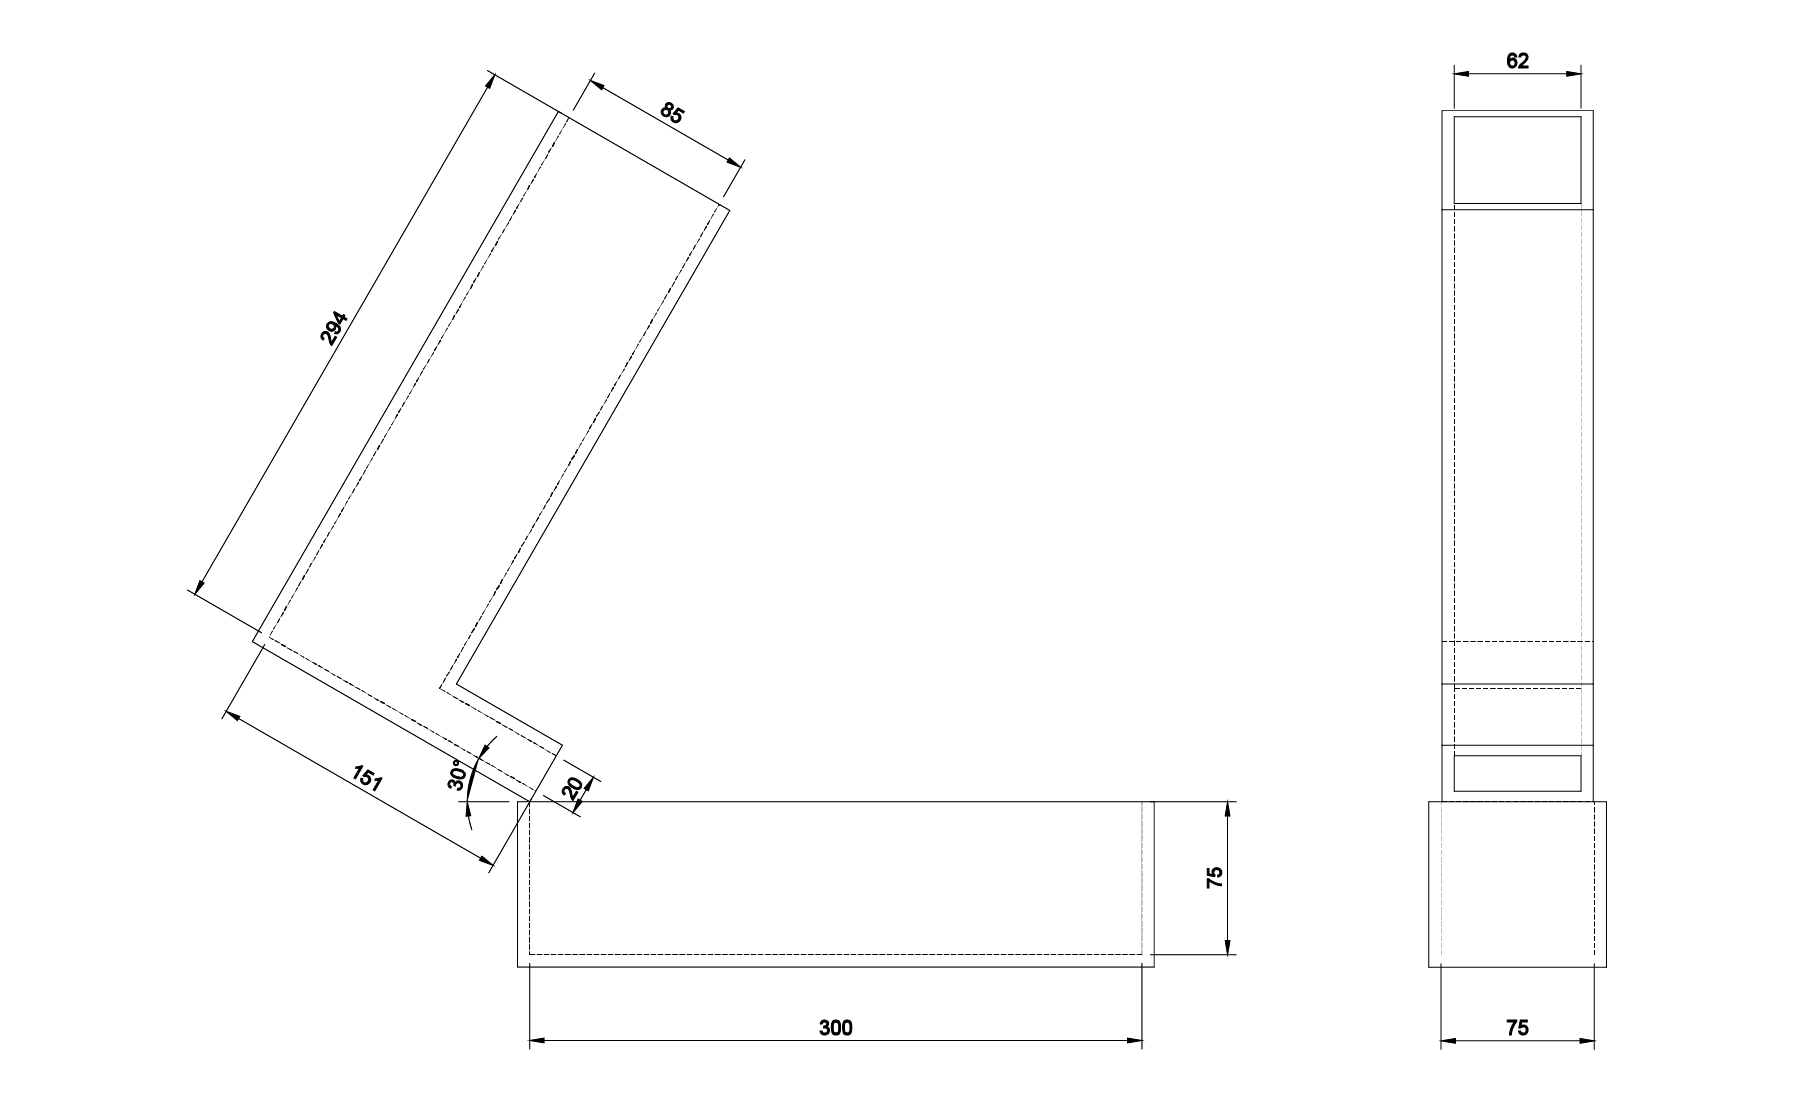
\includegraphics[width=1.0\textwidth]{Ilustraciones/DomainDimentions.png}
    \caption{Dimensioned drawing of the casting device. All dimensions in millimetres.}
    \label{fig:sup_drawing}
\end{figure}

\begin{figure}[htb]
    \centering
    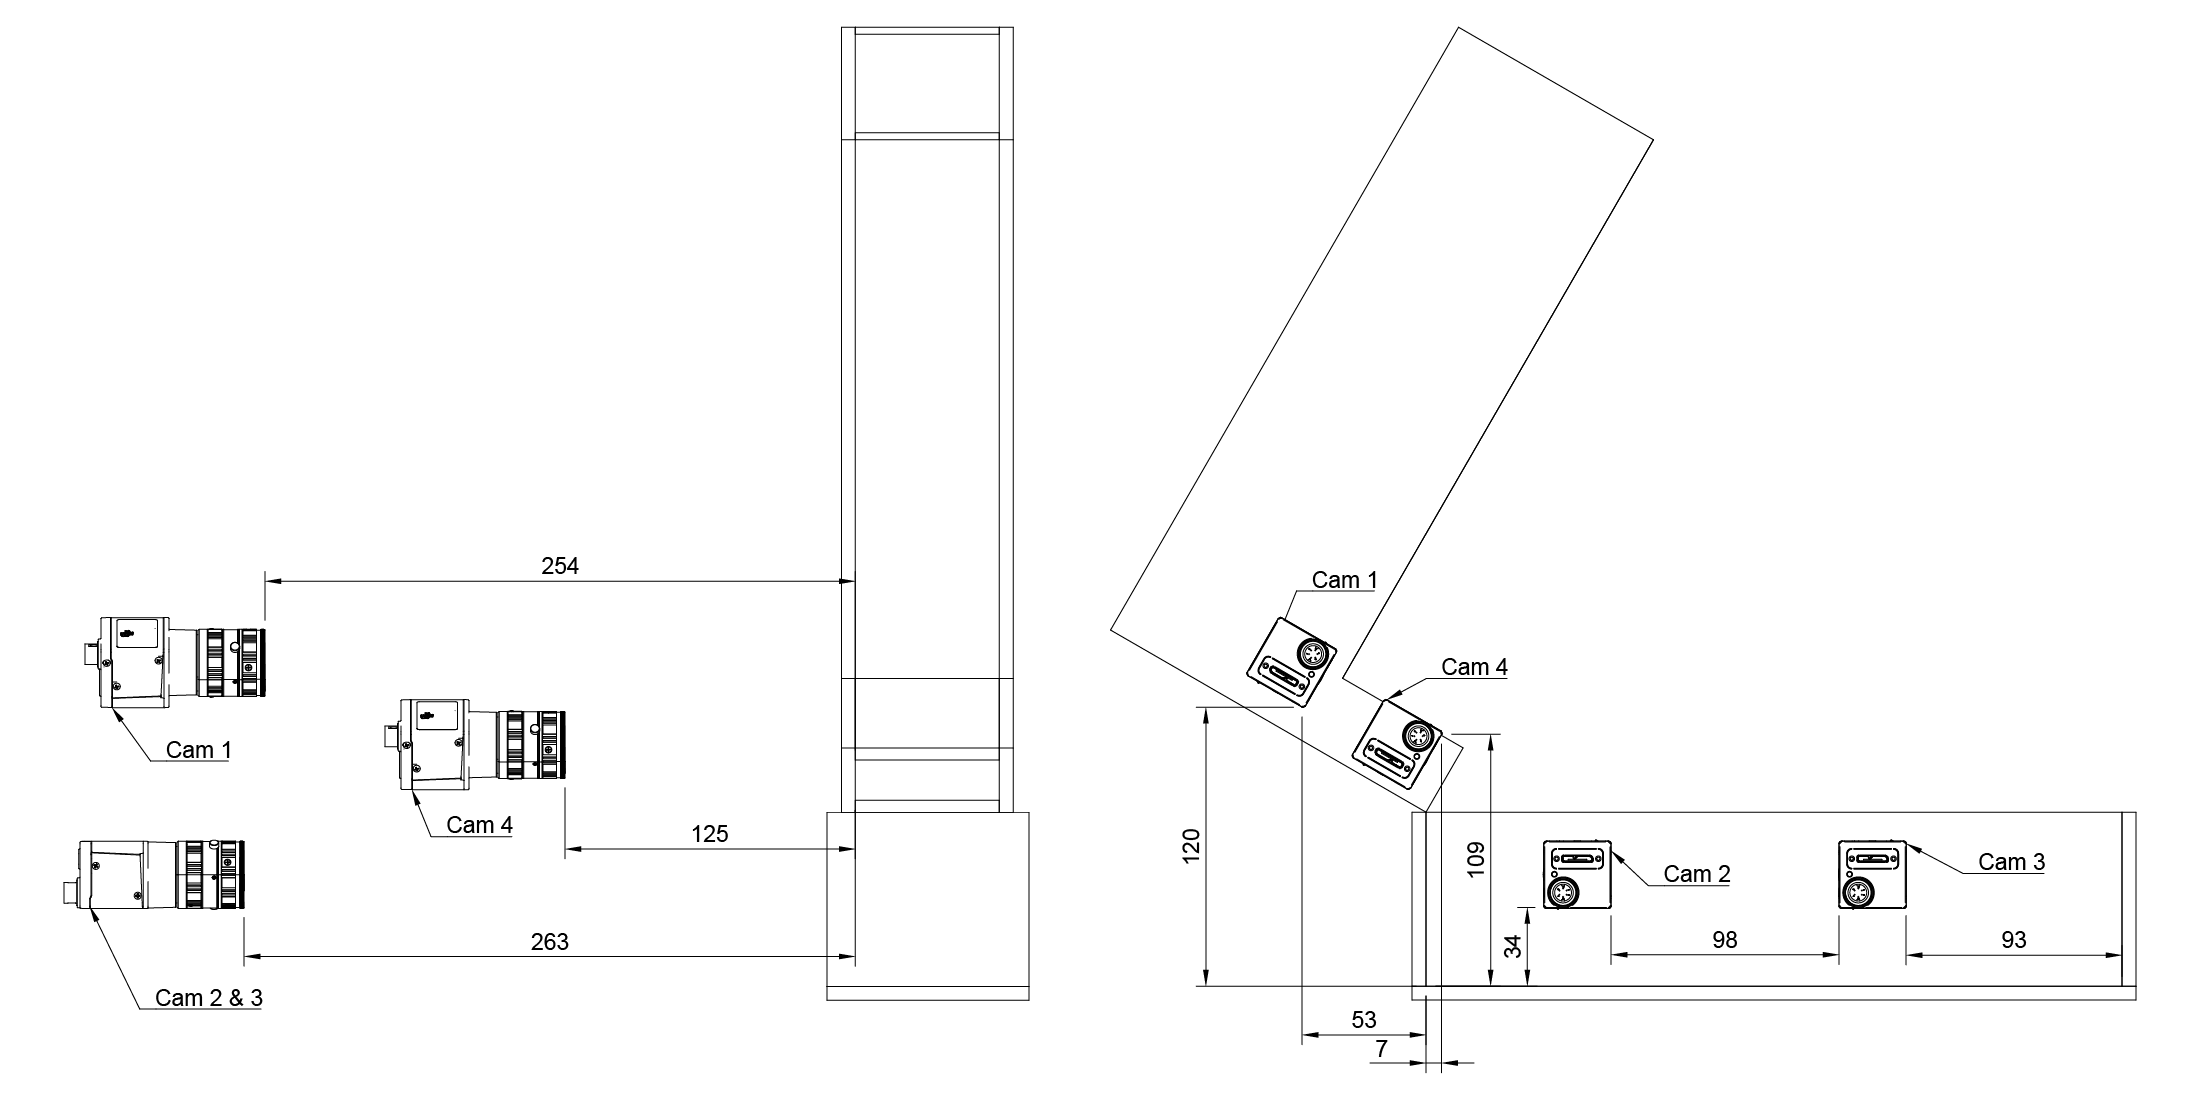
\includegraphics[width=1.0\textwidth]{Ilustraciones/CameraPositions.png}
    \caption{Positions and viewing directions of the four cameras relative to the mold. Distances are in millimetres.}
    \label{fig:sup_cameras}
\end{figure}

\todo{Considerar incluir los renders del montaje ensamblado (Apendice D.3 de la tesis), que muestran el molde, las camaras y la iluminacion sobre la mesa optica desde dos puntos de vista.}


% ============================================================
\section{Record of the gel preparation}
\label{sup:carbopol}
% ============================================================

The yield stress of a Carbopol gel is not a property of its polymer content alone. The polymer is a polyacrylic acid and develops its network only once neutralized: the microgel particles swell as the carboxyl groups ionize, and the yield stress rises with them, reaching its maximum in a band around neutrality and falling away on either side of it. A batch left acidic is a weak gel and a batch overshot is a weak gel, and neither is the material the experiment intends to pour. The pH is therefore not a quality-control formality but the variable through which the rheology reported in the main text is actually set, and a drift in it across batches would be a drift in $\tau_0$, which is the one parameter the two formulations were chosen to contrast.

Table~\ref{tab:sup_ph} reports the pH measured at each of the three stages of the protocol, for the sixteen batches the campaign requires: four dosages, replicated twice, in each of the two matrices. Each value is the average of five points sampled across the mixture, so a batch that had gelled unevenly would be exposed by the spread among those points as well as by the mean.

\begin{table}[htb]
\centering
\caption{Average pH measured during the three stages of the Carbopol preparation, for every batch of the campaign. pH$_1$ is measured after dispersion of the polymer and before neutralization; pH$_2$ after the first dose of 1M NaOH; pH$_3$ after the second dose, and is the value against which the target range of $6.8$ to $7.2$ is checked. Each entry is the average of five points sampled across the mixture.}
\label{tab:sup_ph}
\begin{tabular}{l l c c c}
\toprule
\textbf{Car} & \textbf{Batch} & \textbf{pH$_1$} & \textbf{pH$_2$} & \textbf{pH$_3$} \\
\midrule
\multirow{9}{*}{0.2\%}
 & M70 & 3.56 & 6.89 & 7.07 \\
 & M71 & 3.59 & 6.43 & 6.80 \\
 & M73 & 3.57 & 6.76 & 6.98 \\
 & M74 & 3.56 & 6.75 & 6.90 \\
 & M75 & 3.57 & 6.79 & 6.93 \\
 & M77 & 3.67 & 6.68 & 6.81 \\
 & M80 & 3.59 & 6.93 & 7.08 \\
 & M82 & 3.53 & 6.60 & 6.90 \\
\cmidrule(lr){2-5}
 & Mean $\pm$ s.d. & $3.58\pm0.04$ & $6.73\pm0.16$ & $6.93\pm0.11$ \\
\midrule
\multirow{9}{*}{0.5\%}
 & M83 & 3.37 & 6.39 & 7.10 \\
 & M86 & 3.27 & 6.30 & 7.01 \\
 & M87 & 3.24 & 6.37 & 6.99 \\
 & M91 & 3.28 & 6.33 & 6.90 \\
 & M92 & 3.24 & 6.23 & 6.96 \\
 & M93 & 3.33 & 6.28 & 6.99 \\
 & M94 & 3.28 & 6.28 & 6.91 \\
 & M95 & 3.31 & 6.30 & 6.95 \\
\cmidrule(lr){2-5}
 & Mean $\pm$ s.d. & $3.29\pm0.04$ & $6.31\pm0.05$ & $6.98\pm0.06$ \\
\bottomrule
\end{tabular}
\end{table}

Every batch of both formulations reaches a final pH within the target band, and the spread across batches is narrow, $0.11$ in the softer formulation and $0.06$ in the stiffer one. The two formulations differ systematically in the first two stages, the stiffer gel starting more acidic because it carries more polymer and reaching a lower value after the first dose, but they converge at the third, which is the state in which the material is poured.


% ============================================================
\section{PIV: interrogation parameters and block structure}
\label{sup:piv}
% ============================================================

The two optical techniques process the recorded frames in fundamentally different ways, and the block structure that governs each follows from that difference. PIV correlates a pair of frames and returns the displacement of the tracer pattern between them, so what it must control is the separation between the two frames of a pair: too small and the displacement falls below the resolution of the correlation, too large and the pattern decorrelates. PTV links a sequence of detections and follows each fiber from frame to frame, so what it must control is the interval between consecutive analyzed frames. Both intervals must widen as the flow decelerates, because a spacing that resolves the fast onset produces motions too small to measure once the material has nearly arrested.

Each PIV block is accordingly defined by two quantities. The \emph{inter-pair skip} $s_i$ is the number of frames passed over between the two frames of a correlated pair, and it sets the time separation $\Delta t$ of the pair and hence the tracer displacement the correlation resolves. The \emph{final skip} $s_f$ is the number of frames passed over after a pair is closed and before the next pair begins, and it sets how often a velocity field is produced. Together with the two frames of the pair itself these fix the block length, $b = s_i + s_f + 2$, which is the spacing between the start of one pair and the start of the next, chosen so that the time step $b/\mathrm{fps}$ stays approximately constant within each velocity regime.

\subsection{Interrogation windows}

The velocity field is obtained through a three-pass scheme in which the interrogation window is progressively refined, with a $50\%$ overlap at every pass. Table~\ref{tab:sup_piv_windows} gives the sequence adopted for each camera and formulation. The final window size and the overlap together fix the spacing of the vector grid at half the final window, and that spacing is what sets the amplification of the field error in the spatial derivatives from which the shear rate is computed. It therefore enters the uncertainty on the accumulated strain reported in Sec.~\ref{sup:gamma}.

\begin{table}[htb]
\centering
\caption{PIV interrogation parameters by camera and Carbopol formulation. Window sizes follow a three-pass scheme with $50\%$ overlap at every pass; the final window size and the overlap together fix the spacing of the vector grid.}
\label{tab:sup_piv_windows}
\begin{tabular}{c l c c}
\toprule
\textbf{Camera} & \textbf{Car} & \textbf{Window sizes (px)} & \textbf{Vector spacing (mm)} \\
\midrule
\multirow{2}{*}{1} & 0.2\% & $128 \rightarrow 64 \rightarrow 32$ & 2.00 \\
                   & 0.5\% & $128 \rightarrow 64 \rightarrow 32$ & 2.00 \\
\midrule
\multirow{2}{*}{2} & 0.2\% & $128 \rightarrow 64 \rightarrow 32$ & 2.05 \\
                   & 0.5\% & $64 \rightarrow 32 \rightarrow 16$  & 1.03 \\
\midrule
\multirow{2}{*}{3} & 0.2\% & $64 \rightarrow 32 \rightarrow 16$  & 1.03 \\
                   & 0.5\% & $64 \rightarrow 32 \rightarrow 16$  & 1.03 \\
\midrule
\multirow{2}{*}{4} & 0.2\% & $64 \rightarrow 32 \rightarrow 16$  & 0.75 \\
                   & 0.5\% & $64 \rightarrow 32 \rightarrow 16$  & 0.75 \\
\bottomrule
\end{tabular}
\end{table}

\subsection{The diagnostic that fixes the block boundaries}

The PIV diagnostic is the rate of spurious vectors returned by the normalized median test of the main text. When the inter-pair separation is too small for the flow, the tracer displacement approaches the sub-pixel noise, the correlation returns incoherent vectors, and the spurious rate rises; the appropriate inter-pair skip for a given phase of the filling is the one that minimizes that rate. Figures~\ref{fig:sup_piv_uod_02} and~\ref{fig:sup_piv_uod_05} show, for camera 1 of each matrix, the average velocity recovered under four inter-pair skips together with the corresponding spurious rate. The velocity fields converge as the flow slows, so the choice of skip does not alter the measured field once the flow is in the regime for which the skip is intended, and the spurious rate of each skip is lowest over a distinct interval, moving to later times as the skip grows. The block boundaries are placed where the spurious curve of one skip crosses below that of the next.

\begin{figure}[htb]
    \centering
    \todo{Insertar Fig. B.1 de la tesis.}
    \caption{PIV inter-pair skip sensitivity for Carbopol 0.2\%, camera 1. Left: average velocity under four inter-pair skips, showing convergence as the flow stabilizes. Right: percentage of spurious vectors identified by the normalized median test, on a logarithmic axis. Each skip minimizes the spurious rate over its own interval of the filling, which fixes the transition to the next.}
    \label{fig:sup_piv_uod_02}
\end{figure}

\begin{figure}[htb]
    \centering
    \todo{Insertar Fig. B.2 de la tesis.}
    \caption{PIV inter-pair skip sensitivity for Carbopol 0.5\%, camera 1, over the longer window the stiffer matrix requires. Axes and conventions as in Fig.~\ref{fig:sup_piv_uod_02}.}
    \label{fig:sup_piv_uod_05}
\end{figure}

The onset is the exception and is treated separately. There the velocity is highest, so decorrelation rather than under-resolution is the risk, and the smallest inter-pair skip is retained even where a larger one returns a marginally lower spurious rate, because it is the smallest separation that keeps the tracer pattern within the interrogation window between the two frames.

\subsection{Block structures adopted}

Table~\ref{tab:sup_piv_blocks} gives the resulting structures. Cameras 1 to 3 record at $220$~fps and camera 4, which resolves the fast reorientation at the outlet, at $660$~fps. The near-constant time step of each regime, in the final column, is the quantity the block length is chosen to hold fixed. The first block of camera 3 in the stiffer matrix carries no analysis: the beam it views receives no material for the first eight seconds, so the block is a placeholder spanning that dead interval, and its wide spacing reflects the absence of anything to measure rather than a resolved velocity field.

\begin{table}[htb]
\centering
\caption{PIV block structure by camera and matrix. Each block is defined by its inter-pair skip $s_i$, the number of frames between the two frames of a correlated pair, and its final skip $s_f$, the number of frames between one pair and the next; the block length $s_i + s_f + 2$ sets the time step $\Delta t$. Cameras 1--3 record at $220$~fps, camera 4 at $660$~fps.}
\label{tab:sup_piv_blocks}
\begin{tabular}{l c c c c c c}
\toprule
\textbf{Car} & \textbf{Cam} & $t_0$ [s] & $t_1$ [s] & $s_i$ & $s_f$ & $\Delta t$ [ms] \\
\midrule
\multirow{14}{*}{0.2\%}
 & \multirow{3}{*}{1} &  0.0 &  6.5 & 0 &  9 &  50.0 \\
 &                    &  6.5 & 10.0 & 2 & 18 & 100.0 \\
 &                    & 10.0 & 20.0 & 8 & 12 & 100.0 \\
\cmidrule(lr){2-7}
 & \multirow{4}{*}{2} &  0.0 &  1.5 & 0 &  9 &  50.0 \\
 &                    &  1.5 &  3.0 & 2 & 18 & 100.0 \\
 &                    &  3.0 &  6.0 & 4 & 16 & 100.0 \\
 &                    &  6.0 & 20.0 & 8 & 12 & 100.0 \\
\cmidrule(lr){2-7}
 & \multirow{4}{*}{3} &  0.0 &  2.0 & 0 &  9 &  50.0 \\
 &                    &  2.0 &  5.0 & 2 & 18 & 100.0 \\
 &                    &  5.0 &  7.0 & 4 & 16 & 100.0 \\
 &                    &  7.0 & 20.0 & 8 & 12 & 100.0 \\
\cmidrule(lr){2-7}
 & \multirow{3}{*}{4} &  0.0 &  4.5 & 0 & 20 &  33.3 \\
 &                    &  4.5 &  8.0 & 2 & 18 &  33.3 \\
 &                    &  8.0 & 20.0 & 8 & 12 &  33.3 \\
\midrule
\multirow{13}{*}{0.5\%}
 & \multirow{5}{*}{1} &  0.0 &  0.2 & 0 &  9 &  50.0 \\
 &                    &  0.2 &  5.0 & 1 & 19 & 100.0 \\
 &                    &  5.0 &  8.0 & 2 & 18 & 100.0 \\
 &                    &  8.0 & 15.0 & 4 & 16 & 100.0 \\
 &                    & 15.0 & 40.0 & 8 & 34 & 200.0 \\
\cmidrule(lr){2-7}
 & \multirow{2}{*}{2} &  0.0 & 15.0 &  8 & 12 & 100.0 \\
 &                    & 15.0 & 40.0 & 16 &  4 & 100.0 \\
\cmidrule(lr){2-7}
 & \multirow{2}{*}{3} &  0.0 &  8.0 &  0 & 218 & 1000.0 \\
 &                    &  8.0 & 40.0 & 16 &   4 &  100.0 \\
\cmidrule(lr){2-7}
 & \multirow{4}{*}{4} &  0.0 &  1.5 & 0 &  9 &  16.7 \\
 &                    &  1.5 &  7.5 & 2 & 18 &  33.3 \\
 &                    &  7.5 & 20.0 & 4 & 16 &  33.3 \\
 &                    & 20.0 & 40.0 & 8 & 12 &  33.3 \\
\bottomrule
\end{tabular}
\end{table}


% ============================================================
\section{PTV: sampling intervals and block structure}
\label{sup:ptv}
% ============================================================

The Lagrangian analysis uses cameras 1 to 3, which view the L-shape and the beam; camera 4, dedicated to the outlet, does not enter the fiber tracking. Each PTV block is defined by a single skip, the number of frames passed over between two analyzed frames, since the tracking is continuous and Lagrangian and simply follows each fiber through the frames it retains.

\subsection{The displacement diagnostic}

The PTV diagnostic is the pair displacement $\Delta x$, the distance a fiber travels between two analyzed frames, against a floor of $0.25$~mm below which the displacement can no longer be separated from the localization noise in the fiber position and the link becomes unreliable. Figures~\ref{fig:sup_ptv_disp_02} and~\ref{fig:sup_ptv_disp_05} show $\Delta x$ under a sequence of skips: each skip holds the displacement above the floor over its own interval, and the point at which a given skip approaches the floor is the point at which the next, larger skip takes over.

\begin{figure}[htb]
    \centering
    \todo{Insertar Fig. B.3 de la tesis.}
    \caption{PTV skip sensitivity for Carbopol 0.2\%. Pair displacement $\Delta x$, the distance a fiber travels between analyzed frames, under four skips, against the floor of $0.25$~mm (dashed). Each skip is drawn bold over the interval in which it is adopted; below the floor the displacement is indistinguishable from the localization noise.}
    \label{fig:sup_ptv_disp_02}
\end{figure}

\begin{figure}[htb]
    \centering
    \todo{Insertar Fig. B.4 de la tesis.}
    \caption{PTV skip sensitivity for Carbopol 0.5\%. Axes and conventions as in Fig.~\ref{fig:sup_ptv_disp_02}.}
    \label{fig:sup_ptv_disp_05}
\end{figure}

\subsection{Block structures adopted}

Table~\ref{tab:sup_ptv_blocks} gives the structures, together with the search radius $\Delta x_{\max}$ within which a fiber is sought in the next analyzed frame, tightened as the flow slows and the displacements shorten.

\begin{table}[htb]
\centering
\caption{PTV block structure by camera and matrix, for the three cameras used in the fiber tracking. Each block is defined by its skip, the number of frames passed over between analyzed frames, and the maximum linking distance $\Delta x_{\max}$. All three cameras record at $220$~fps.}
\label{tab:sup_ptv_blocks}
\begin{tabular}{l c c c c c}
\toprule
\textbf{Car} & \textbf{Cam} & $t_0$ [s] & $t_1$ [s] & \textbf{Skip} & $\Delta x_{\max}$ [mm] \\
\midrule
\multirow{13}{*}{0.2\%}
 & \multirow{4}{*}{1} & 0.0 &  2.5 & 0 & 3.0 \\
 &                    & 2.5 &  5.0 & 2 & 2.5 \\
 &                    & 5.0 &  8.0 & 4 & 2.0 \\
 &                    & 8.0 & 20.0 & 8 & 2.0 \\
\cmidrule(lr){2-6}
 & \multirow{4}{*}{2} & 0.0 &  3.0 & 0 & 3.0 \\
 &                    & 3.0 &  5.0 & 2 & 2.5 \\
 &                    & 5.0 &  8.0 & 4 & 2.0 \\
 &                    & 8.0 & 20.0 & 8 & 2.0 \\
\cmidrule(lr){2-6}
 & \multirow{5}{*}{3} & 0.0 &  0.5 & 10 & 3.0 \\
 &                    & 0.5 &  1.5 &  0 & 3.0 \\
 &                    & 1.5 &  3.0 &  2 & 2.5 \\
 &                    & 3.0 &  6.0 &  4 & 2.0 \\
 &                    & 6.0 & 20.0 &  8 & 2.0 \\
\midrule
\multirow{12}{*}{0.5\%}
 & \multirow{5}{*}{1} &  0.0 &  0.2 &  0 & 3.0 \\
 &                    &  0.2 &  3.0 &  2 & 2.5 \\
 &                    &  3.0 &  8.0 &  4 & 2.5 \\
 &                    &  8.0 & 15.0 &  8 & 2.5 \\
 &                    & 15.0 & 40.0 & 16 & 2.5 \\
\cmidrule(lr){2-6}
 & \multirow{4}{*}{2} &  0.0 &  0.2 &  0 & 3.0 \\
 &                    &  0.2 &  3.0 &  4 & 2.5 \\
 &                    &  3.0 & 15.0 &  8 & 2.5 \\
 &                    & 15.0 & 40.0 & 16 & 2.5 \\
\cmidrule(lr){2-6}
 & \multirow{3}{*}{3} &  0.0 & 10.0 & 10 & 3.0 \\
 &                    & 10.0 & 15.0 &  8 & 2.5 \\
 &                    & 15.0 & 40.0 & 16 & 2.5 \\
\bottomrule
\end{tabular}
\end{table}


% ============================================================
\section{Reduction in computational cost}
\label{sup:cost}
% ============================================================

The block structure reduces the computational load of both techniques, but the quantity reduced differs between them, and the two are reported on their own terms rather than on a common one.

For PIV the cost is the number of correlated pairs, since each pair is one cross-correlation regardless of how the frames within it are spaced. A block of length $b = s_i + s_f + 2$ produces one pair and the next pair begins $b$ frames later, so a phase spanning $F$ frames yields $F/b$ pairs against the $F$ that a correlation of every consecutive pair would require. It is the final skip and not the inter-pair skip that governs this saving: widening the separation within a pair changes the displacement resolved but not the number of pairs, whereas widening the gap between pairs is what reduces their count. For PTV the cost is the number of frames analyzed, since the tracking processes each retained frame once, and a block of skip $s$ over $F$ frames analyzes $F/(s+1)$ of them.

\begin{table}[htb]
\centering
\caption{Reduction in computational load relative to processing every frame: for PIV, the reduction in the number of correlated pairs; for PTV, the reduction in the number of frames analyzed. PTV uses cameras 1--3 only.}
\label{tab:sup_cost}
\begin{tabular}{c c c c c}
\toprule
 & \multicolumn{2}{c}{\textbf{PIV (pairs)}} & \multicolumn{2}{c}{\textbf{PTV (frames)}} \\
\cmidrule(lr){2-3}\cmidrule(lr){4-5}
\textbf{Camera} & 0.2\% [\%] & 0.5\% [\%] & 0.2\% [\%] & 0.5\% [\%] \\
\midrule
1 & 94.0 & 96.9 & 73.7 & 89.0 \\
2 & 95.1 & 95.5 & 72.0 & 91.1 \\
3 & 95.0 & 96.3 & 81.5 & 92.7 \\
4 & 95.5 & 95.3 & --   & --   \\
\midrule
Overall & 95.1 & 95.7 & 75.7 & 90.9 \\
\bottomrule
\end{tabular}
\end{table}

The PIV analysis processes about one pair in twenty of what an exhaustive correlation would, a reduction above $94\%$ for every camera and both matrices, because even the fastest phase spaces its pairs widely and the long arrested phase spaces them wider still. The PTV reduction is smaller and more variable, between $72$ and $93\%$, and it is smallest in the softer matrix, whose filling is brief and largely fast enough to demand the smallest skips, and largest in the stiffer matrix, whose long slow arrest is tracked at the widest spacing. In both techniques and both matrices the saving is what makes the full campaign tractable without sacrificing the temporal resolution the fast early phase requires.


% ============================================================
\section{Uncertainty on the accumulated strain}
\label{sup:gamma}
% ============================================================

The main text states the uncertainty on $\Gamma$ as a single figure and gives the two features of the integration that produce it. This section resolves both cell by cell.

\subsection{Where the deformation is delivered}

Figure~\ref{fig:sup_weight} gives the cumulative fraction of the accumulated strain against the fraction of the traverse covered, for every destination cell. The curves rise steeply and then flatten, which is the signature of a yield stress confining the shear to a thin layer at the entry: the first third of the path delivers between $81\%$ and $86\%$ of the final $\Gamma$ in every case.

\begin{figure}[htb]
    \centering
    \todo{Insertar: peso acumulado de la deformacion contra fraccion del trayecto, una curva por celda de destino. Datos en B\_peso\_acumulado.csv.}
    \caption{Cumulative fraction of the accumulated strain against the fraction of the traverse covered, for each destination cell of the beam. The first third of the path delivers between $81\%$ and $86\%$ of the final value in every case.}
    \label{fig:sup_weight}
\end{figure}

\subsection{Uncertainty resolved by cell}

Table~\ref{tab:sup_gamma_uncertainty} reports, for each dosage and cell, the fraction of $\Gamma$ delivered within the first third of the traverse, the number of integration segments, the random component of the uncertainty after averaging over the trajectory realizations of the cell, and the systematic component. The random component falls below one percent everywhere, so the uncertainty on $\Gamma$ is set by the systematic term, which is common to every cell and every dosage and therefore rescales the horizontal axis of the fits without displacing the points relative to one another.

\begin{table}[htb]
\centering
\caption{Uncertainty on the accumulated strain, by fiber dosage and beam cell. $w_{30}$ is the fraction of $\Gamma$ delivered within the first third of the traverse; $n_{seg}$ the number of integration segments; $\delta_{rand}$ the random component after averaging over the trajectory realizations of the cell; $\delta_{sys}$ the systematic component, common to every cell and dosage.}
\label{tab:sup_gamma_uncertainty}
\begin{tabular}{l l S[table-format=2.1] S[table-format=4.0] S[table-format=1.2] S[table-format=1.1] S[table-format=2.1]}
\toprule
\textbf{$N$} & \textbf{Cell} &
  \multicolumn{1}{c}{$\Gamma_{beam}$} &
  \multicolumn{1}{c}{$n_{seg}$} &
  \multicolumn{1}{c}{$w_{30}$} &
  \multicolumn{1}{c}{\makecell{$\delta_{rand}$ \\ (\%)}} &
  \multicolumn{1}{c}{\makecell{$\delta_{sys}$ \\ (\%)}} \\
\midrule
\multirow{5}{*}{750}
 & r1c1 & 15.8 &  651 & 0.82 & 0.3 & 10.6 \\
 & r1c2 & 24.6 & 1280 & 0.82 & 0.6 & 10.6 \\
 & r2c1 & 16.1 &  651 & 0.84 & 0.4 & 10.6 \\
 & r2c2 & 28.0 & 1292 & 0.83 & 0.5 & 10.6 \\
 & r2c3 & 35.5 & 1835 & 0.81 & 0.5 & 10.6 \\
\midrule
\multirow{5}{*}{1500}
 & r1c1 & 17.7 &  652 & 0.83 & 0.3 & 10.6 \\
 & r1c2 & 28.2 & 1287 & 0.82 & 0.9 & 10.6 \\
 & r2c1 & 17.3 &  652 & 0.86 & 0.4 & 10.6 \\
 & r2c2 & 32.2 & 1295 & 0.85 & 0.5 & 10.6 \\
 & r2c3 & 41.1 & 1847 & 0.82 & 0.6 & 10.6 \\
\midrule
\multirow{5}{*}{3000}
 & r1c1 & 17.8 &  653 & 0.82 & 0.3 & 10.6 \\
 & r1c2 & 27.3 & 1286 & 0.82 & 0.6 & 10.6 \\
 & r2c1 & 17.2 &  653 & 0.86 & 0.3 & 10.6 \\
 & r2c2 & 32.3 & 1296 & 0.84 & 0.5 & 10.6 \\
 & r2c3 & 41.9 & 1857 & 0.82 & 0.5 & 10.6 \\
\bottomrule
\end{tabular}
\end{table}

\subsection{Repeatability of the fiber-free control}

The four independent acquisitions of the fiber-free control in Carbopol $0.2\%$, two batches supplying two acquisitions each, are the only replicated condition of the campaign and therefore the only direct measurement of repeatability. Table~\ref{tab:sup_gamma_replicates} reports the value of $\Gamma$ each acquisition returns in each cell, together with the coefficient of variation over the four. The replicates share a calibration, so they probe the random component of the uncertainty alone, and the level at which they agree is consistent with the estimate of Table~\ref{tab:sup_gamma_uncertainty}.

\begin{table}[htb]
\centering
\caption{Accumulated strain returned by each of the four acquisitions of the fiber-free control in Carbopol $0.2\%$, by beam cell, with the mean, the standard deviation and the coefficient of variation over the four.}
\label{tab:sup_gamma_replicates}
\begin{tabular}{l S[table-format=2.2] S[table-format=2.2] S[table-format=2.2] S[table-format=2.2] S[table-format=2.2] S[table-format=1.2] S[table-format=1.1]}
\toprule
\textbf{Cell} &
  \multicolumn{4}{c}{\textbf{Acquisition}} &
  \multicolumn{1}{c}{\textbf{Mean}} &
  \multicolumn{1}{c}{\textbf{SD}} &
  \multicolumn{1}{c}{\makecell{\textbf{CV} \\ (\%)}} \\
\cmidrule(lr){2-5}
 & \multicolumn{1}{c}{1} & \multicolumn{1}{c}{2} & \multicolumn{1}{c}{3} & \multicolumn{1}{c}{4} & & & \\
\midrule
r1c1 & 22.83 & 22.22 & 22.74 & 22.77 & 22.64 & 0.28 & 1.3 \\
r1c2 & 33.64 & 33.42 & 33.82 & 33.54 & 33.60 & 0.17 & 0.5 \\
r2c1 & 18.40 & 19.23 & 19.94 & 19.06 & 19.16 & 0.63 & 3.3 \\
r2c2 & 31.06 & 31.67 & 33.14 & 31.70 & 31.89 & 0.88 & 2.8 \\
r2c3 & 37.35 & 38.51 & 39.78 & 37.96 & 38.40 & 1.03 & 2.7 \\
\bottomrule
\end{tabular}
\end{table}


% ============================================================
\section{Effect sizes resolved by zone}
\label{sup:zonal}
% ============================================================

The main text reports, for each variable and each flow stage, the largest effect the fiber content exerts anywhere in the domain, together with the zone in which it is found. This section gives the effect in every zone. These tables are the source from which the summary table of the main text is drawn, collected here because the argument rests on a claim about the distribution of the effect and not merely its peak: that the influence of the fiber content is regional, concentrated where the geometry forces a change in the flow, and that a domain-averaged measurement would report its absence. A table of maxima cannot test that claim; these can.

\subsection{Protocol}

Each cell of each table reports one analysis of covariance, run within a single zone, flow stage and rheological matrix, with time as a continuous covariate and the fiber content as the factor of interest. The covariate is not optional: the filling is transient, so a zone passes through very different flow conditions as the mold fills, and comparing raw means across dosages would confound the effect of the fibers with the shared temporal trend of the flow. The two numbers reported are the partial eta squared, the share of variance the fiber content explains once that trend is removed, and the $p$ value of the same term.

The two answer different questions, and the tables mark them separately. An entry carries an asterisk when its effect size reaches the relevance threshold of $\eta^2 = 0.02$, with further asterisks at $0.10$ and $0.30$, and is set in bold when that relevant effect is also significant at $p < 0.05$. Bold is the case in which the fiber content is reported as acting. The distinction matters because the samples run to thousands of observations, so the test can return a vanishingly small $p$ for effects far too small to carry any physical consequence; such entries are read, correctly, as the absence of a relevant effect. Significance alone is never taken as evidence that the fibers act.

The zones are not equally populated in the two matrices. Carbopol $0.5\%$ arrests while the beam is still half empty, so the cells of its distal columns receive little or no material. The tables are therefore restricted, in each matrix, to the zones the flow actually reaches: a zone is retained when the carrier establishes a resolved velocity field within it and the final state deposits a countable population of fibers. The two criteria agree, and are applied identically to the Eulerian and Lagrangian tables, so both cover six zones in the stiffer matrix against eight in the softer one.

\subsection{Eulerian variables}

Tables~\ref{tab:sup_zonal_euler_02} and~\ref{tab:sup_zonal_euler_05} report the effect of the fiber content on the speed $|\bm{u}|$ and the vorticity magnitude $|\zeta|$ of the carrier, measured by PIV.

Two features carry the argument of the main text. The first is that the fiber content acts on the speed almost everywhere the carrier is moving: in Carbopol $0.5\%$ the effect on $|\bm{u}|$ is relevant in sixteen of the eighteen zone-stage combinations, and it grows as the flow decelerates, reaching $\eta^2 = 0.525$ at the beam inlet in the quasi-steady stage. The fibers slow the carrier, and do so systematically. The second is that the vorticity does not follow: where the effect on the speed is strongest, in the stiff matrix, the effect on the vorticity never exceeds $0.160$. That separation is the observation on which the rotational decoupling rests.

\begin{table}[htb]
\centering
\caption{Effect of fiber content $N$ on the Eulerian variables, Carbopol $0.2\%$, by zone and flow stage. Each variable reports the partial eta squared and the covariate-adjusted $p$ value of the fiber-content term. Bold marks a relevant and significant effect ($\eta^2 \geq 0.02$ and $p < 0.05$); asterisks mark the effect-size bands alone. $^{*}\,\eta^2 \geq 0.02$; $^{**}\,\eta^2 \geq 0.10$; $^{***}\,\eta^2 \geq 0.30$.}
\label{tab:sup_zonal_euler_02}
\begin{tabular}{l l r l r l}
\toprule
 & & \multicolumn{2}{c}{$|\bm{u}|$} & \multicolumn{2}{c}{$|\zeta|$} \\
\cmidrule(lr){3-4}\cmidrule(lr){5-6}
\textbf{Stage} & \textbf{Zone} & $\eta^2$ & $p$ & $\eta^2$ & $p$ \\
\midrule
\multirow{8}{*}{Onset}
 & Z1   & 0.004                 & 0.191        & \textbf{0.283}$^{**}$ & \pv{9}{-47} \\
 & Z2   & \textbf{0.049}$^{*}$  & \pv{5}{-23}  & 0.015                 & \pv{6}{-6} \\
 & Z3   & 0.015                 & 0.010        & 0.001                 & 0.717 \\
 & r1c1 & \textbf{0.165}$^{**}$ & \pv{4}{-26}  & 0.005                 & 0.353 \\
 & r1c2 & 0.012                 & \pv{5}{-7}   & \textbf{0.032}$^{*}$  & 0.044 \\
 & r2c1 & \textbf{0.057}$^{*}$  & \pv{4}{-16}  & 0.003                 & 0.211 \\
 & r2c2 & 0.003                 & 0.222        & 0.002                 & 0.405 \\
 & r2c3 & \textbf{0.022}$^{*}$  & \pv{1}{-7}   & 0.015                 & \pv{1}{-5} \\
\midrule
\multirow{8}{*}{Transition}
 & Z1   & \textbf{0.057}$^{*}$  & \pv{2}{-146} & \textbf{0.228}$^{**}$ & \pv{9}{-42} \\
 & Z2   & \textbf{0.102}$^{**}$ & \pv{3}{-146} & \textbf{0.036}$^{*}$  & \pv{2}{-31} \\
 & Z3   & 0.010                 & \pv{9}{-28}  & 0.004                 & $<0.001$ \\
 & r1c1 & \textbf{0.021}$^{*}$  & \pv{2}{-71}  & 0.004                 & \pv{3}{-6} \\
 & r1c2 & \textbf{0.022}$^{*}$  & \pv{2}{-73}  & 0.003                 & 0.040 \\
 & r2c1 & \textbf{0.031}$^{*}$  & \pv{2}{-82}  & 0.019                 & \pv{4}{-18} \\
 & r2c2 & 0.017                 & \pv{6}{-38}  & 0.005                 & 0.001 \\
 & r2c3 & \textbf{0.045}$^{*}$  & \pv{6}{-105} & \textbf{0.065}$^{*}$  & \pv{2}{-32} \\
\midrule
\multirow{8}{*}{Quasi-steady}
 & Z1   & \textbf{0.021}$^{*}$  & \pv{2}{-54}  & \textbf{0.020}$^{*}$  & \pv{2}{-64} \\
 & Z2   & \textbf{0.049}$^{*}$  & \pv{5}{-143} & 0.004                 & \pv{6}{-22} \\
 & Z3   & 0.010                 & \pv{9}{-50}  & 0.000                 & 0.424 \\
 & r1c1 & 0.020                 & \pv{1}{-117} & 0.001                 & 0.145 \\
 & r1c2 & \textbf{0.023}$^{*}$  & \pv{2}{-20}  & \textbf{0.042}$^{*}$  & \pv{6}{-41} \\
 & r2c1 & 0.014                 & \pv{1}{-83}  & 0.003                 & \pv{1}{-9} \\
 & r2c2 & 0.015                 & \pv{3}{-71}  & 0.002                 & 0.026 \\
 & r2c3 & \textbf{0.048}$^{*}$  & \pv{1}{-28}  & \textbf{0.061}$^{*}$  & \pv{8}{-44} \\
\bottomrule
\end{tabular}
\end{table}

\begin{table}[htb]
\centering
\caption{Effect of fiber content $N$ on the Eulerian variables, Carbopol $0.5\%$, by zone and flow stage. The stiffer matrix arrests before filling the third column of the beam, so its distal cells receive no material and are absent from the table. Conventions as in Table~\ref{tab:sup_zonal_euler_02}.}
\label{tab:sup_zonal_euler_05}
\begin{tabular}{l l r l r l}
\toprule
 & & \multicolumn{2}{c}{$|\bm{u}|$} & \multicolumn{2}{c}{$|\zeta|$} \\
\cmidrule(lr){3-4}\cmidrule(lr){5-6}
\textbf{Stage} & \textbf{Zone} & $\eta^2$ & $p$ & $\eta^2$ & $p$ \\
\midrule
\multirow{6}{*}{Onset}
 & Z1   & \textbf{0.070}$^{*}$   & \pv{2}{-21}  & \textbf{0.084}$^{*}$  & \pv{2}{-25} \\
 & Z2   & \textbf{0.292}$^{**}$  & \pv{4}{-245} & 0.009                 & \pv{1}{-7} \\
 & Z3   & \textbf{0.097}$^{*}$   & \pv{3}{-72}  & \textbf{0.094}$^{*}$  & \pv{2}{-83} \\
 & r1c1 & \textbf{0.037}$^{*}$   & \pv{3}{-35}  & 0.005                 & \pv{4}{-8} \\
 & r2c1 & \textbf{0.027}$^{*}$   & \pv{7}{-25}  & 0.005                 & \pv{2}{-9} \\
 & r2c2 & \textbf{0.050}$^{*}$   & \pv{2}{-27}  & \textbf{0.052}$^{*}$  & \pv{7}{-25} \\
\midrule
\multirow{6}{*}{Transition}
 & Z1   & \textbf{0.116}$^{**}$  & \pv{2}{-100} & \textbf{0.047}$^{*}$  & \pv{2}{-74} \\
 & Z2   & \textbf{0.434}$^{***}$ & $<10^{-300}$ & \textbf{0.062}$^{*}$  & \pv{4}{-64} \\
 & Z3   & \textbf{0.044}$^{*}$   & \pv{2}{-146} & \textbf{0.095}$^{*}$  & \pv{7}{-66} \\
 & r1c1 & \textbf{0.131}$^{**}$  & $<10^{-300}$ & 0.005                 & \pv{4}{-13} \\
 & r2c1 & \textbf{0.070}$^{*}$   & $<10^{-300}$ & \textbf{0.034}$^{*}$  & \pv{1}{-37} \\
 & r2c2 & 0.017                  & \pv{6}{-91}  & \textbf{0.030}$^{*}$  & \pv{1}{-34} \\
\midrule
\multirow{6}{*}{Quasi-steady}
 & Z1   & 0.013                  & \pv{1}{-90}  & \textbf{0.077}$^{*}$  & $<10^{-300}$ \\
 & Z2   & \textbf{0.150}$^{**}$  & $<10^{-300}$ & 0.011                 & \pv{3}{-75} \\
 & Z3   & \textbf{0.024}$^{*}$   & \pv{6}{-319} & \textbf{0.070}$^{*}$  & \pv{3}{-286} \\
 & r1c1 & \textbf{0.525}$^{***}$ & \pv{1}{-75}  & \textbf{0.098}$^{*}$  & \pv{2}{-10} \\
 & r2c1 & \textbf{0.142}$^{**}$  & \pv{3}{-269} & \textbf{0.108}$^{**}$ & \pv{2}{-125} \\
 & r2c2 & \textbf{0.067}$^{*}$   & \pv{6}{-104} & \textbf{0.160}$^{**}$ & \pv{8}{-231} \\
\bottomrule
\end{tabular}
\end{table}

\subsection{Lagrangian variables}

Tables~\ref{tab:sup_zonal_lagrange_02} and~\ref{tab:sup_zonal_lagrange_05} report the effect of the fiber content on the fiber speed $|\bm{v}|$, the angular velocity $|\omega|$ and the orientation order $\eta_1$, measured by PTV, over the same zones the Eulerian analysis resolves.

The angular velocity is the variable these tables single out. It carries a relevant and significant effect in most zones and stages of both matrices, and its peaks are among the largest anywhere in the dataset, reaching $\eta^2 = 0.502$ in the vertical arm of the softer matrix during the transition and $\eta^2 = 0.430$ in the first beam column of the stiffer one once the flow has settled. The orientation order climbs higher still, to $\eta^2 = 0.713$ at the beam inlet of the softer matrix in the quasi-steady stage, the single largest response of the whole dataset. Read against the Eulerian tables, where the vorticity of the carrier responds far more weakly to how many fibers it carries, this is the rotational decoupling of the main text: the fibers turn faster as their number grows, and the fluid carrying them does so far less.

\begin{table*}[htb]
\centering
\caption{Effect of fiber content $N$ on the Lagrangian variables, Carbopol $0.2\%$, by zone and flow stage. The table covers the same zones as the Eulerian analysis of Table~\ref{tab:sup_zonal_euler_02}. Conventions as in Table~\ref{tab:sup_zonal_euler_02}.}
\label{tab:sup_zonal_lagrange_02}
\begin{tabular}{l l r l r l r l}
\toprule
 & & \multicolumn{2}{c}{$|\bm{v}|$} & \multicolumn{2}{c}{$|\omega|$} & \multicolumn{2}{c}{$\eta_1$} \\
\cmidrule(lr){3-4}\cmidrule(lr){5-6}\cmidrule(lr){7-8}
\textbf{Stage} & \textbf{Zone} & $\eta^2$ & $p$ & $\eta^2$ & $p$ & $\eta^2$ & $p$ \\
\midrule
\multirow{8}{*}{Onset}
 & Z1   & \textbf{0.043}$^{*}$  & \pv{6}{-9}   & \textbf{0.426}$^{***}$ & \pv{3}{-102} & \textbf{0.180}$^{**}$  & \pv{7}{-43} \\
 & Z2   & 0.018                 & \pv{4}{-6}   & \textbf{0.143}$^{**}$  & \pv{1}{-52}  & \textbf{0.284}$^{**}$  & \pv{2}{-101} \\
 & Z3   & \textbf{0.037}$^{*}$  & \pv{3}{-12}  & \textbf{0.093}$^{*}$   & \pv{4}{-31}  & \textbf{0.140}$^{**}$  & \pv{5}{-49} \\
 & r1c1 & \textbf{0.072}$^{*}$  & \pv{1}{-26}  & 0.003                  & 0.191        & 0.015                  & 0.002 \\
 & r1c2 & \textbf{0.146}$^{**}$ & \pv{4}{-65}  & 0.019                  & 0.168        & \textbf{0.173}$^{**}$  & 0.009 \\
 & r2c1 & 0.020                 & \pv{2}{-6}   & \textbf{0.086}$^{*}$   & \pv{1}{-23}  & \textbf{0.076}$^{*}$   & \pv{1}{-19} \\
 & r2c2 & \textbf{0.165}$^{**}$ & \pv{2}{-92}  & \textbf{0.183}$^{**}$  & \pv{1}{-88}  & \textbf{0.046}$^{*}$   & \pv{7}{-20} \\
 & r2c3 & 0.020                 & \pv{2}{-8}   & \textbf{0.026}$^{*}$   & \pv{4}{-5}   & \textbf{0.234}$^{**}$  & \pv{3}{-25} \\
\midrule
\multirow{8}{*}{Transition}
 & Z1   & \textbf{0.279}$^{**}$ & \pv{2}{-249} & \textbf{0.502}$^{***}$ & $<10^{-300}$ & \textbf{0.141}$^{**}$  & \pv{2}{-106} \\
 & Z2   & \textbf{0.145}$^{**}$ & \pv{4}{-207} & \textbf{0.178}$^{**}$  & \pv{1}{-211} & \textbf{0.082}$^{*}$   & \pv{2}{-48} \\
 & Z3   & \textbf{0.044}$^{*}$  & \pv{6}{-45}  & 0.007                  & \pv{8}{-8}   & 0.006                  & $<0.001$ \\
 & r1c1 & \textbf{0.093}$^{*}$  & \pv{1}{-145} & \textbf{0.090}$^{*}$   & \pv{9}{-131} & 0.002                  & 0.076 \\
 & r1c2 & 0.017                 & \pv{6}{-12}  & 0.015                  & \pv{5}{-9}   & 0.007                  & 0.002 \\
 & r2c1 & \textbf{0.221}$^{**}$ & $<10^{-300}$ & \textbf{0.201}$^{**}$  & \pv{3}{-274} & \textbf{0.161}$^{**}$  & \pv{1}{-113} \\
 & r2c2 & \textbf{0.086}$^{*}$  & \pv{7}{-113} & \textbf{0.089}$^{*}$   & \pv{8}{-102} & 0.015                  & \pv{4}{-10} \\
 & r2c3 & \textbf{0.075}$^{*}$  & \pv{3}{-33}  & \textbf{0.226}$^{**}$  & \pv{5}{-80}  & \textbf{0.057}$^{*}$   & \pv{2}{-17} \\
\midrule
\multirow{8}{*}{Quasi-steady}
 & Z1   & \textbf{0.031}$^{*}$   & \pv{6}{-43}  & \textbf{0.054}$^{*}$   & \pv{9}{-77}  & \textbf{0.069}$^{*}$   & \pv{7}{-57} \\
 & Z2   & \textbf{0.020}$^{*}$   & \pv{1}{-34}  & \textbf{0.054}$^{*}$   & \pv{7}{-96}  & 0.015                  & \pv{6}{-15} \\
 & Z3   & 0.012                  & \pv{5}{-19}  & \textbf{0.031}$^{*}$   & \pv{2}{-26}  & \textbf{0.053}$^{*}$   & \pv{2}{-37} \\
 & r1c1 & \textbf{0.068}$^{*}$   & \pv{3}{-82}  & \textbf{0.239}$^{**}$  & \pv{2}{-247} & \textbf{0.278}$^{**}$  & \pv{8}{-176} \\
 & r1c2 & \textbf{0.133}$^{**}$  & \pv{4}{-78}  & \textbf{0.203}$^{**}$  & \pv{1}{-117} & \textbf{0.105}$^{**}$  & \pv{1}{-53} \\
 & r2c1 & \textbf{0.046}$^{*}$   & \pv{5}{-69}  & \textbf{0.071}$^{*}$   & \pv{8}{-107} & \textbf{0.713}$^{***}$ & $<10^{-300}$ \\
 & r2c2 & \textbf{0.173}$^{**}$  & \pv{6}{-302} & \textbf{0.358}$^{***}$ & $<10^{-300}$ & \textbf{0.359}$^{***}$ & $<10^{-300}$ \\
 & r2c3 & \textbf{0.396}$^{***}$ & \pv{3}{-136} & \textbf{0.323}$^{***}$ & \pv{4}{-97}  & \textbf{0.187}$^{**}$  & \pv{1}{-50} \\
\bottomrule
\end{tabular}
\end{table*}

\begin{table*}[htb]
\centering
\caption{Effect of fiber content $N$ on the Lagrangian variables, Carbopol $0.5\%$, by zone and flow stage. As in the Eulerian analysis, the distal columns the arresting flow never fills are absent; the six zones listed are those in which the carrier establishes a resolved field and a countable fiber population is tracked. Conventions as in Table~\ref{tab:sup_zonal_euler_02}.}
\label{tab:sup_zonal_lagrange_05}
\begin{tabular}{l l r l r l r l}
\toprule
 & & \multicolumn{2}{c}{$|\bm{v}|$} & \multicolumn{2}{c}{$|\omega|$} & \multicolumn{2}{c}{$\eta_1$} \\
\cmidrule(lr){3-4}\cmidrule(lr){5-6}\cmidrule(lr){7-8}
\textbf{Stage} & \textbf{Zone} & $\eta^2$ & $p$ & $\eta^2$ & $p$ & $\eta^2$ & $p$ \\
\midrule
\multirow{6}{*}{Onset}
 & Z1   & \textbf{0.161}$^{**}$ & \pv{8}{-68}  & \textbf{0.333}$^{***}$ & \pv{5}{-134} & \textbf{0.407}$^{***}$ & \pv{1}{-120} \\
 & Z2   & \textbf{0.050}$^{*}$  & \pv{1}{-61}  & \textbf{0.219}$^{**}$  & \pv{8}{-262} & \textbf{0.186}$^{**}$  & \pv{1}{-113} \\
 & Z3   & 0.018                 & \pv{2}{-11}  & \textbf{0.110}$^{**}$  & \pv{3}{-95}  & \textbf{0.095}$^{*}$   & \pv{2}{-56} \\
 & r1c1 & 0.003                 & 0.024        & 0.015                  & \pv{1}{-6}   & \textbf{0.039}$^{*}$   & \pv{7}{-16} \\
 & r2c1 & 0.000                 & 0.973        & 0.009                  & \pv{3}{-5}   & \textbf{0.048}$^{*}$   & \pv{3}{-26} \\
 & r2c2 & \textbf{0.029}$^{*}$  & \pv{4}{-11}  & \textbf{0.025}$^{*}$   & \pv{4}{-5}   & 0.010                  & 0.094 \\
\midrule
\multirow{6}{*}{Transition}
 & Z1   & \textbf{0.091}$^{*}$  & \pv{2}{-123} & \textbf{0.327}$^{***}$ & $<10^{-300}$ & \textbf{0.354}$^{***}$ & \pv{7}{-232} \\
 & Z2   & 0.005                 & 0.009        & \textbf{0.126}$^{**}$  & \pv{7}{-56}  & \textbf{0.378}$^{***}$ & \pv{2}{-123} \\
 & Z3   & 0.004                 & 0.033        & \textbf{0.025}$^{*}$   & \pv{9}{-10}  & \textbf{0.105}$^{**}$  & \pv{2}{-32} \\
 & r1c1 & \textbf{0.030}$^{*}$  & \pv{1}{-12}  & \textbf{0.230}$^{**}$  & \pv{2}{-93}  & \textbf{0.109}$^{**}$  & \pv{2}{-40} \\
 & r2c1 & \textbf{0.057}$^{*}$  & \pv{1}{-18}  & \textbf{0.138}$^{**}$  & \pv{8}{-39}  & \textbf{0.523}$^{***}$ & \pv{2}{-165} \\
 & r2c2 & 0.007                 & 0.008        & 0.018                  & \pv{2}{-5}   & 0.009                  & 0.006 \\
\midrule
\multirow{6}{*}{Quasi-steady}
 & Z1   & \textbf{0.083}$^{*}$   & \pv{6}{-102} & \textbf{0.285}$^{**}$  & \pv{1}{-273} & 0.012                  & \pv{1}{-6} \\
 & Z2   & \textbf{0.022}$^{*}$   & \pv{2}{-17}  & \textbf{0.234}$^{**}$  & \pv{7}{-161} & \textbf{0.384}$^{***}$ & \pv{3}{-237} \\
 & Z3   & 0.000                  & 0.559        & \textbf{0.060}$^{*}$   & \pv{3}{-31}  & 0.000                  & 0.694 \\
 & r1c1 & \textbf{0.280}$^{**}$  & \pv{3}{-15}  & \textbf{0.247}$^{**}$  & \pv{2}{-13}  & \textbf{0.306}$^{***}$ & \pv{3}{-16} \\
 & r2c1 & \textbf{0.368}$^{***}$ & \pv{1}{-95}  & \textbf{0.430}$^{***}$ & \pv{2}{-121} & \textbf{0.340}$^{***}$ & \pv{1}{-84} \\
 & r2c2 & \textbf{0.029}$^{*}$   & \pv{1}{-5}   & \textbf{0.026}$^{*}$   & \pv{5}{-5}   & \textbf{0.052}$^{*}$   & \pv{1}{-10} \\
\bottomrule
\end{tabular}
\end{table*}

\subsection{Reading the distribution}

Two properties of the whole set of tables bear on the interpretation of the main text, and neither is visible in a table of maxima.

The first is that the effect is regional. In every matrix and for every variable, zones in which the fiber content acts strongly sit alongside zones in which it does not act at all, and the strong ones are those where the geometry forces a change in the flow: the elbow, where the material turns; the beam inlet, where it lands; and the vertical arm, where the descent first develops. This is why the effect nearly vanishes when the domain is pooled, and why the pooled figure is the less informative of the two. Pooling places the variance between a plug descending the arm and a nearly arrested beam cell into the error term, and that variance dominates any effect the fibers could exert. The pooled value therefore establishes only that the fiber content is small relative to the spatial heterogeneity of the flow, which holds for any flow through this geometry and is not a statement about the fibers.

The second is that the effect broadly strengthens as the flow decelerates. Reading down the three stages of a column, the entries tend to rise from the onset toward the quasi-steady stage, and the strongest responses of the dataset are recorded in these later stages, once the flow has settled or is settling into arrest. This is what would be expected if the fibers act by adding hydrodynamic resistance to a carrier already near its yield threshold, since the same increment of effective consistency matters more where the material is barely moving than where it descends under gravity, and it is one reason the analysis of the final state is conducted on the arrested configuration rather than on the flow that produced it.

\subsection{Flow stage boundaries}

The criterion that locates the stage boundaries is described in the main text. Its numerical parameters are collected here: the median velocity of each zone is smoothed with a centred moving average of $0.25$~s; the peak is located after excluding the first $0.5$~s, which is dominated by the transient of the gate release; the onset ends when the smoothed velocity first falls below $60\%$ of that peak; and the quasi-steady stage begins when it falls below $15\%$ of the peak in Carbopol $0.2\%$ and $30\%$ in Carbopol $0.5\%$. A minimum onset duration of $0.5$~s is enforced, and a zone holding fewer than fifty valid control timestamps inherits its boundaries from the larger geometric region to which it belongs.

The asymmetry of the lower threshold between the two formulations is physical rather than procedural. The stiffer gel carries a higher yield stress and arrests earlier, so its flow comes to rest at a residual velocity that remains a larger fraction of the peak it once reached; a single low threshold would locate the onset of the quasi-steady stage beyond the point at which that material has already stopped moving.


% ============================================================
\section{Additional descriptors of the arrested population}
\label{sup:finalstate}
% ============================================================

The main text reports the orientation of the arrested population and states that its spatial dispersion does not respond to the fiber content. This section gives the dispersion measurements on which that statement rests, together with two instantaneous quantities that the main text does not use to support a conclusion.

\subsection{Spatial dispersion of the arrested fibers}

The dispersion index $\Lambda$ compares the radius of gyration of the fiber centroids within a cell with that of a uniform arrangement over the same region, so that $\Lambda = 1$ denotes a uniform arrangement, $\Lambda < 1$ clustering, and $\Lambda > 1$ an arrangement displaced toward the boundaries of the cell. Figure~\ref{fig:sup_lambda} reports it cell by cell.

Within the beam the dispersion is governed by the rheology and not by the fiber content. Carbopol $0.2\%$ reaches values at or slightly above unity in the cells of the lower row, whereas Carbopol $0.5\%$ remains below unity in every populated cell. The contrast follows from how each matrix arrests: the stiffer gel stops flowing while still advancing and locks the fibers wherever they happen to be, preserving whatever clustering they carried out of the L-shape, while the softer gel keeps flowing for longer, so the fibers are carried and rearranged more completely before the material sets.

\begin{figure}[htb]
    \centering
    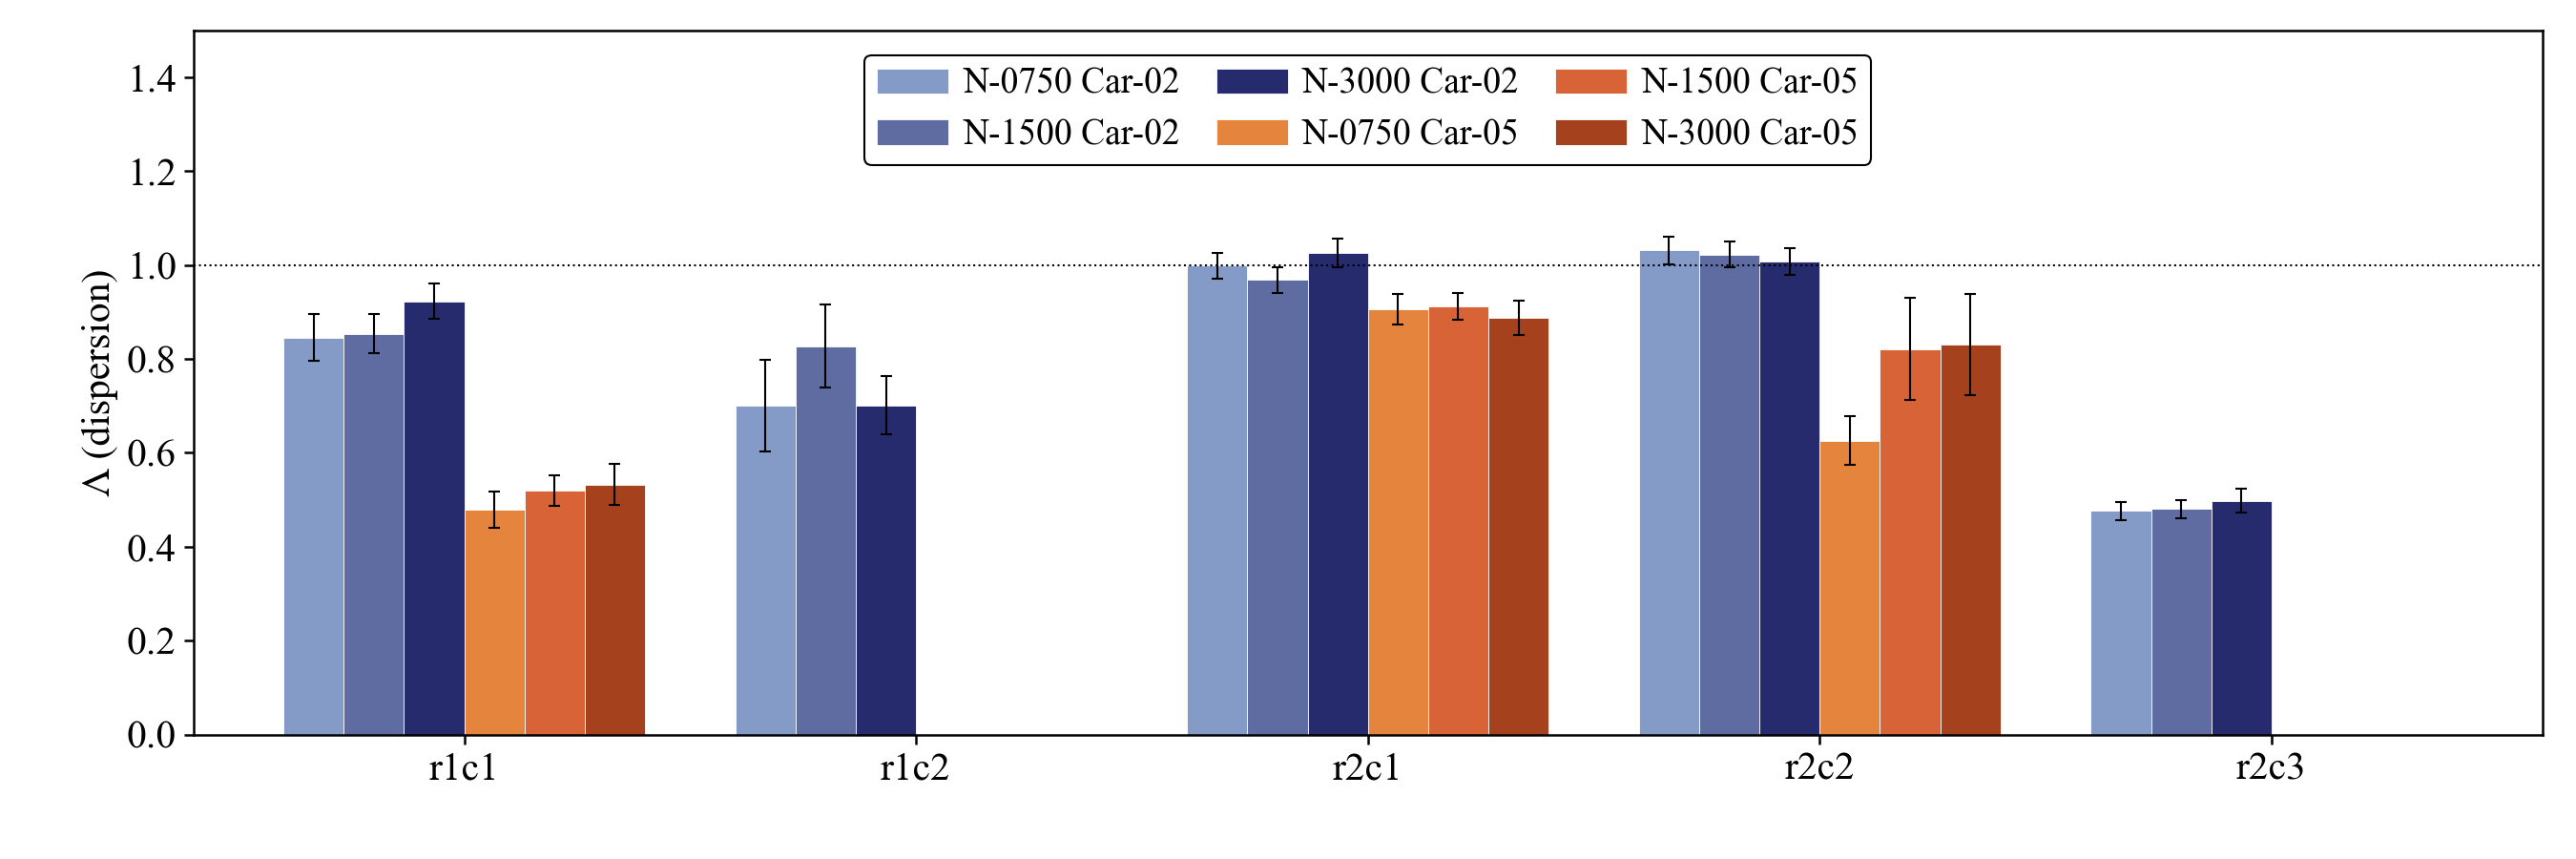
\includegraphics[width=1.0\textwidth]{Ilustraciones/A12_viga_carbopol_dispersion.png}
    \caption{Dispersion index $\Lambda$ of the arrested fiber centroids in each beam cell, grouped by fiber dosage and formulation. The dotted line marks $\Lambda = 1$, the value of a spatially uniform arrangement; lower values indicate clustering. Error bars span one standard deviation.}
    \label{fig:sup_lambda}
\end{figure}

One region falls outside this account and is reported here rather than omitted. In the vertical arm of the softer matrix the fiber content does act on the dispersion, with $\eta^2 = 0.302$ at $p = 0.003$, which is the largest effect the fiber content exerts on any quantity of the dataset. The vertical arm is not part of the cast element, and the measurement cannot separate two explanations of equal standing: the effect may describe how a denser suspension redistributes its fibers as it descends, or it may describe how the fibers were introduced into the reservoir before release. The result is therefore recorded and not interpreted.

\subsection{Instantaneous fiber speed and orientation order}

Figures~\ref{fig:sup_v} and~\ref{fig:sup_eta_inst} give the spatial distribution of the fiber speed and of the instantaneous orientation order across zones and dosages, completing the set of Lagrangian quantities whose effect sizes the main text tabulates. Neither supports a conclusion of the main text on its own: the fiber speed cannot be compared with the fluid speed because the two techniques sample different depths, and the instantaneous order does not survive pooling.

\begin{figure}[htb]
    \centering
    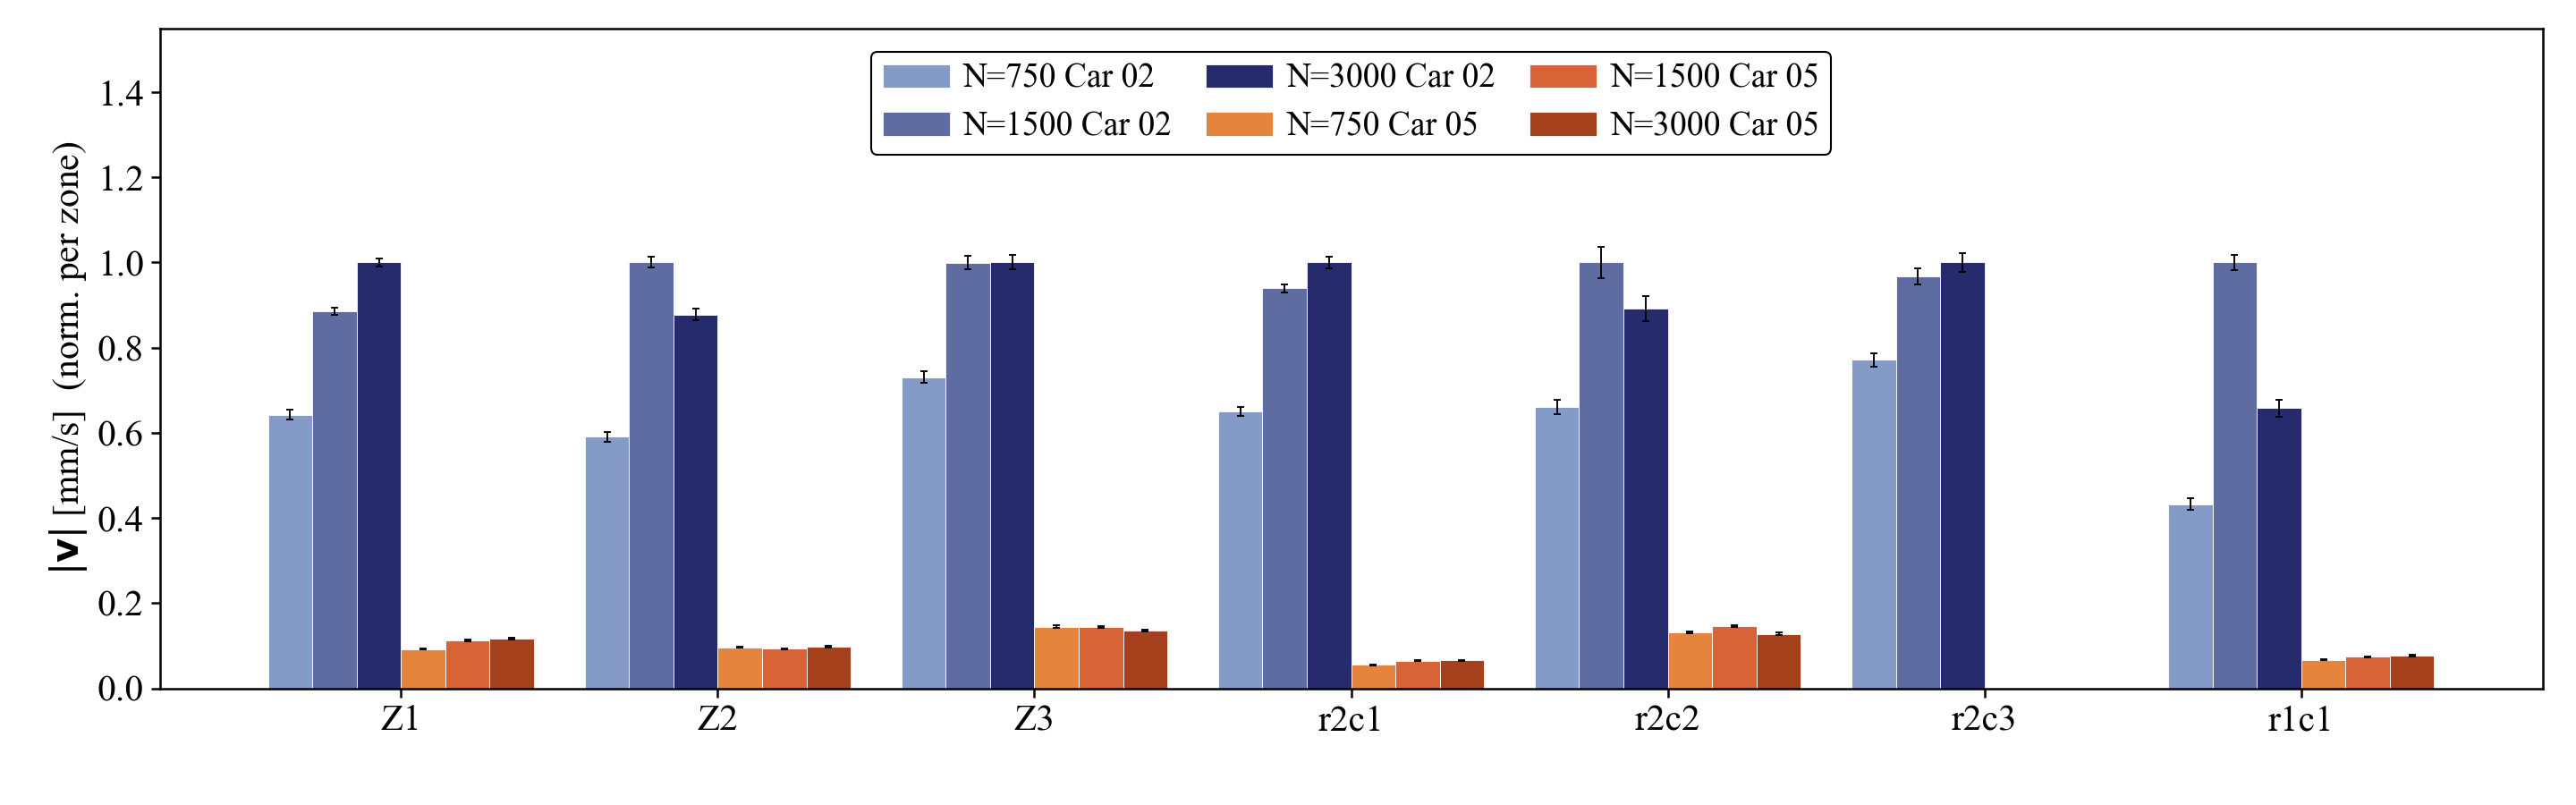
\includegraphics[width=1.0\textwidth]{Ilustraciones/ENT_ptv_speed.png}
    \caption{Spatial distribution of the fiber speed $|\bm{v}|$ across zones and fiber contents during the transition stage, for Carbopol 0.2\% (top) and 0.5\% (bottom).}
    \label{fig:sup_v}
\end{figure}

\begin{figure}[htb]
    \centering
    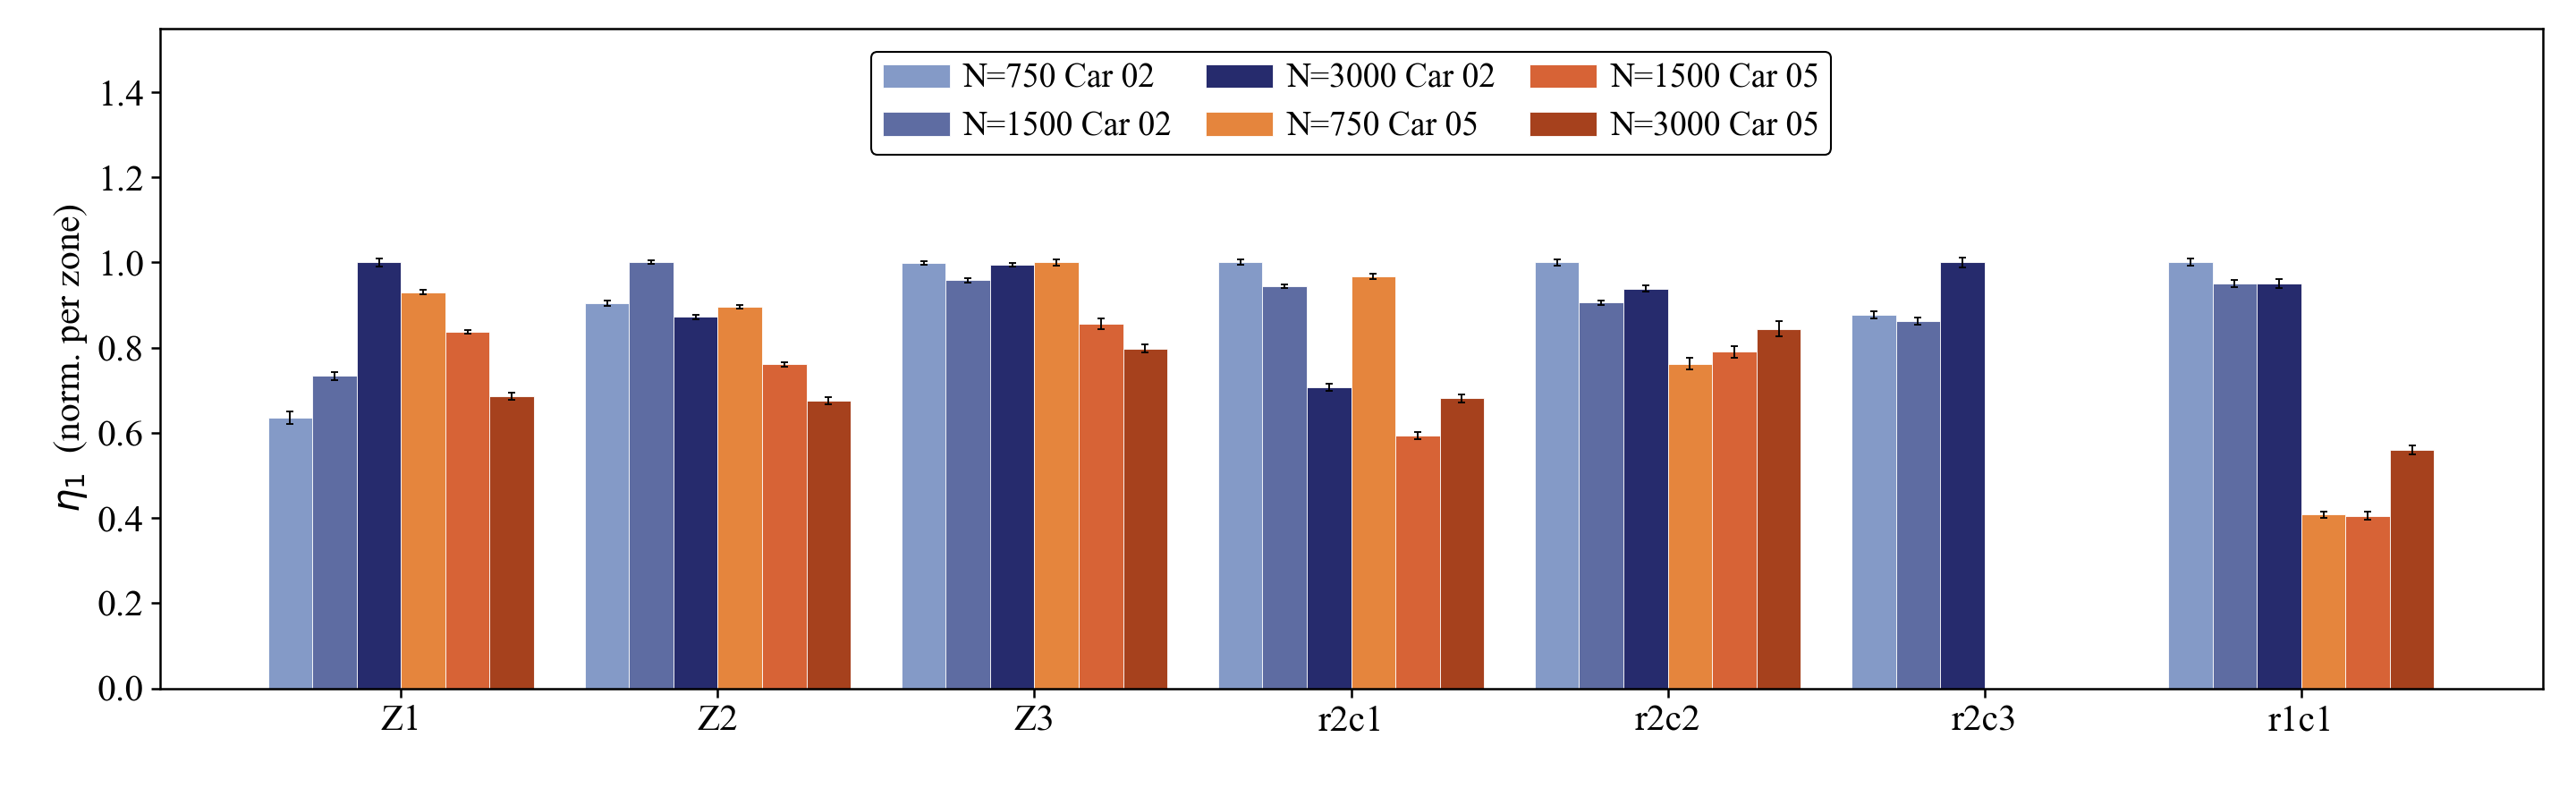
\includegraphics[width=1.0\textwidth]{Ilustraciones/ENT_ptv_eta1.png}
    \caption{Spatial distribution of the instantaneous orientation order $\eta_1$ across zones and fiber contents during the transition stage, for Carbopol 0.2\% (top) and 0.5\% (bottom).}
    \label{fig:sup_eta_inst}
\end{figure}

\subsection{Photographs of the arrested elements}

Figure~\ref{fig:sup_arrested} shows the beam after arrest at each dosage and in both formulations. The images are the direct visual counterpart of the descriptors reported above, and they make explicit the difference in spreading between the two matrices: the softer gel fills the beam over its full length, while the stiffer one arrests before the third column is reached.

\begin{figure}[htb]
    \centering
    \todo{Insertar Apendice F.4 de la tesis: fotografias de los elementos detenidos para cada dosis y ambas formulaciones.}
    \caption{The beam after arrest, at each fiber dosage and in both Carbopol formulations.}
    \label{fig:sup_arrested}
\end{figure}

\end{document}